% This goes at the from of the file - you can select different things here like 12pt, 11pt, paper size, double sided etc.

\documentclass[a4paper,11pt]{article}

% Packages for different settings - there are many of these you can access by googling (item you want and latex).
\usepackage{amsfonts}
\usepackage{pifont}
\usepackage{graphicx}
\usepackage{amsmath}
\usepackage{enumerate}
\usepackage{epsfig}
\usepackage{latexsym}
\usepackage{amssymb}
\usepackage{color}
\usepackage{amscd}
\usepackage{natbib}
\usepackage{multirow}
\usepackage{graphicx}
\usepackage{lscape}
\usepackage{float}
\usepackage{bm}
\usepackage{listings}
\usepackage[hypcap]{caption}

%%%%%%%%%%%%%%%%%%%%%%%%%%%%%%%%
% paper margins settings.
\pagestyle{plain}  
\oddsidemargin0cm
\hoffset-1cm
\voffset-0.5cm
\topmargin-1.4cm 
\textheight25cm \textwidth18cm \parindent0.5cm
%%%%%%%%%%%%%%%%%%%%%%%%%%%%%%%%


\begin{document}
\title{Assignment 2: MATH3911}
\author{Alexander Kwok$^{1}$  
\\$^{[1]}${\small email:
z3332883@zmail.unsw.edu.au; } 
}

\date{\textbf{Assignment 2:} Version from \today }

\maketitle
This assignment is my own work. I have read and understood the University Rules in respect to Student Academic Misconduct.
\section*{Question 1}
\begin{enumerate}[(a)]
	\item
		It is given that $X_1,X_2, ...,X_{10}$ are $i.i.d$ distributed random variables from $N(\mu,4)$ with a density function as follow:\\
		\[
		f(x;\mu) = \frac{1}{2\sqrt{2\pi}}e^{-\frac{(x-\mu)^2}{8}}
		\]
		Therefore the likelihood function of $X_i$ is
		\begin{align*}
		L(x;\mu)&=\prod^{10}_{i=1} f(x_i;\mu)\\
		&= \bigg( \frac{1}{2\sqrt{2\pi}}  \bigg)^{10} exp\bigg(-\frac{1}{8}\sum^{10}_{i=1}(x_i-\mu)^2   \bigg)\\
		&= \bigg( \frac{1}{2\sqrt{2\pi}}  \bigg)^{10} exp\bigg(-\frac{1}{8}\sum^{10}_{i=1}(x_i^2-2x_i\mu+\mu^2)   \bigg)\\
		&= \bigg( \frac{1}{2\sqrt{2\pi}}  \bigg)^{10} exp\bigg(-\frac{1}{8}\sum^{10}_{i=1}x_i^2 \bigg)exp\bigg(\frac{1}{4}\mu\sum^{10}_{i=1}x_i   \bigg)exp\bigg(-\frac{10}{8}\mu^2   \bigg)\\
		&= \bigg( \frac{1}{2\sqrt{2\pi}}  \bigg)^{10} exp\bigg(-\frac{1}{8}\sum^{10}_{i=1}x_i^2 \bigg)exp\bigg(\frac{1}{4}\mu\sum^{10}_{i=1}x_i   \bigg)exp\bigg(-\frac{5}{4}\mu^2   \bigg)
		\end{align*}
		Then the likelihood ratio can be written as
		\begin{align*}
		\frac{L(x;\mu_2)}{L(x;\mu_1)}&=\frac{\bigg( \frac{1}{2\sqrt{2\pi}} \bigg)^{10}exp\bigg(-\frac{1}{8}\sum^{10}_{i=1}x_i^2 \bigg)exp\bigg(\frac{1}{4}\mu_2\sum^{10}_{i=1}x_i   \bigg)exp\bigg(-\frac{5}{4}\mu_2^2   \bigg)
}{\bigg(\frac{1}{2\sqrt{2\pi}}  \bigg)^{10}exp\bigg(-\frac{1}{8}\sum^{10}_{i=1}x_i^2 \bigg)exp\bigg(\frac{1}{4}\mu_1\sum^{10}_{i=1}x_i   \bigg)exp\bigg(-\frac{5}{4}\mu_1^2   \bigg)
}\\
		&= exp\bigg(\frac{1}{4}[\mu_2-\mu_1]\sum^{10}_{i=1}x_i \bigg)exp\bigg(-\frac{5}{4}(\mu_2^2 - \mu_1^2)   \bigg)
		\end{align*}
		which is a non-decreasing function of $\sum^{10}_{i=1} X_i$ for any fixed $\mu_1$ and $\mu_2$, with $\mu_1 < \mu_2$. Therefore, the joint density of $X_1,X_2, ...,X_{10}$ has monotone likelihood ratio in $T(X) = \sum^{10}_{i=1} X_i$.
	\item
		By rearranging the likelihood ratio as
		\begin{align*}
		L(x;\mu)&= \bigg( \frac{1}{2\sqrt{2\pi}}  \bigg)^{10} exp\bigg(-\frac{1}{8}\sum^{10}_{i=1}x_i^2 \bigg)exp\bigg(\frac{1}{4}\mu\sum^{10}_{i=1}x_i   \bigg)exp\bigg(-\frac{5}{4}\mu^2   \bigg)\\
		&= \bigg( \frac{1}{2\sqrt{2\pi}}e^{-\frac{1}{8}\mu^2}  \bigg)^{10}\bigg(\prod^{10}_{i=1}e^{-\frac{1}{8}x_i^2} \bigg)exp\bigg(\frac{1}{4}\mu\sum^{10}_{i=1}x_i   \bigg)
		\end{align*}
		which is in the form
		\begin{align*}
		(a(\mu))^n\bigg( \prod^{n}_{i=1}b(x_i) \bigg)exp\bigg(c(\mu) \sum^n_{i=1}d(x_i)  \bigg)
		\end{align*}
		with $T(X) = \sum^{10}_{i=1}d(X_i) = \sum^{10}_{i=1} X_i$.\\
		Therefore, the UMP unbiased size $\alpha = 0.1$ test of $H_0:\mu=1$ versus $H_1:\mu \neq1$ is 
		\[
		\varphi^*(X)= \left\{ 
			\begin{array}{rcl}
			1 & \mbox{if}
			&  T(X)<c_1 \mbox{ or } T(X)>c_2 \\ 0 & \mbox{if} & c_1\le T(X) \le c_2 \\
			\end{array}\right.
		\]
	where the constants $c_i (i=1,2)$, satisfy the conditions:
		\begin{equation}\label{az1}	
			E_{\mu=1}[\varphi^*(X)] = 0.1
		\end{equation}
		\begin{equation}\label{az2}	
			\bigg[ \frac{\partial}{\partial\mu}E_{\mu}[\varphi^*(X)]\bigg]_{\mu=1} = 0
		\end{equation}
		Note that
		\[
		T(X) = \sum^{10}_{i=1}X_i \sim N(10\mu,40)
		\]
		and
		\[
		\frac{T(X)-10\mu}{\sqrt{40}} \sim N(0,1)
		\]
	Therefore, the power function can be deduced as
		\begin{align*}
			E_{\mu}[\varphi^*(X)]&= P[\varphi^*(X)=1]\\
			&=P[T(X)<c_1)+P(T(X)>c_2]\\
			&=P\bigg(\frac{T(X)-10\mu}{\sqrt{40}}<\frac{c_1-10\mu}{\sqrt{40}}\bigg)+P\bigg(\frac{T(X)-10\mu}{\sqrt{40}}>\frac{c_2-10\mu}{\sqrt{40}}\bigg)\\
			&= \Phi\bigg( \frac{c_1-10\mu}{2\sqrt{10}}\bigg) +1 - \Phi \bigg(  \frac{c_2-10\mu}{2\sqrt{10}}\bigg)
		\end{align*}
	As a result, we have
		\begin{align*}
			\frac{\partial}{\partial\mu}E_{\mu}[\varphi^*(X)] &= -\frac{10}{2\sqrt{10}} \Phi'\bigg( \frac{c_1-10\mu}{2\sqrt{10}}\bigg)+ \frac{10}{2\sqrt{10}} \Phi'\bigg(  \frac{c_2-10\mu}{2\sqrt{10}}\bigg)\\
			&= -\frac{\sqrt{10}}{2} \Phi'\bigg( \frac{c_1-10\mu}{2\sqrt{10}}\bigg)+ \frac{\sqrt{10}}{2}\Phi'\bigg(  \frac{c_2-10\mu}{2\sqrt{10}}\bigg)
		\end{align*}
	where
		\[
			\Phi'(z) = \frac{d}{dz}\Phi(z) =\frac{1}{\sqrt{2\pi}} e^{-\frac{1}{2}z^2} 
		\]
	which is the standard normal density function.\\
	Use condition ~\eqref{az2}, we have 
		\begin{align*}
			\bigg[ \frac{\partial}{\partial\mu}E_{\mu}[\varphi^*(X)]\bigg]_{\mu=1} &= 0\\
			-\frac{\sqrt{10}}{2} \Phi'\bigg( \frac{c_1-10}{2\sqrt{10}}\bigg)+ \frac{\sqrt{10}}{2}\Phi'\bigg(  \frac{c_2-10}{2\sqrt{10}}\bigg)&=0\\
			\phi\bigg(  \frac{c_2-10}{2\sqrt{10}}\bigg)&=\phi\bigg( \frac{c_1-10}{2\sqrt{10}}\bigg)
		\end{align*}
	Since $c_1 \ne c_2$ and using the fact that density of normal distribution is symmetric around zero, then
		\begin{align*}
			\frac{c_2-10}{2\sqrt{10}}&= -\frac{c_1-10}{2\sqrt{10}}\\
			c_1 &=  20 -c_2
		\end{align*}
	Then substitute $c_1 =  20 -c_2$ to \eqref{az1} and using the fact that $\Phi(-z) = 1- \Phi(z)$,
		\begin{align*}
			E_{\mu=1}[\varphi^*(X)] &= 0.1\\
			\Phi\bigg( \frac{c_1-10}{2\sqrt{10}}\bigg) +1 - \Phi \bigg(  \frac{c_2-10}{2\sqrt{10}}\bigg)  &= 0.1\\
			\Phi\bigg( \frac{ 20 -c_2-10}{2\sqrt{10}}\bigg) +1 - \Phi \bigg(  \frac{c_2-10}{2\sqrt{10}}\bigg) &= 0.1\\
			\Phi\bigg( \frac{  -c_2+10}{2\sqrt{10}}\bigg) +1 - \Phi \bigg(  \frac{c_2-10}{2\sqrt{10}}\bigg) &= 0.1\\
			1-\Phi\bigg( \frac{  c_2-10}{2\sqrt{10}}\bigg) +1 - \Phi \bigg(  \frac{c_2-10}{2\sqrt{10}}\bigg) &= 0.1\\
			1- \Phi \bigg(  \frac{c_2-10}{2\sqrt{10}}\bigg) &= 0.05\\
			 \Phi \bigg(  \frac{c_2-10}{2\sqrt{10}}\bigg) &= 0.95\\
			 \frac{c_2-10}{2\sqrt{10}} &= \Phi^{-1}(0.95)\\
			c_2 &= 10+2\sqrt{10} \times \Phi^{-1}(0.95)
		\end{align*}
	Therefore,
		\[
			c_2 \approx10+2\sqrt{10} \times(1.644854) =  20.40297  \mbox{ and } c_1 = 20-c_2 \approx -0.40297
		\]
	Then the UMP unbiased size $\alpha = 0.1$ is 
		  \[
		\varphi^*(X)= \left\{ 
			\begin{array}{rcl}
			1 & \mbox{if}
			&  T(X)<-0.40297 \mbox{ or } T(X)>20.40297 \\ 0 & \mbox{if} & -0.40297\le T(X) \le 20.40297 \\
			\end{array}\right.
		\]
	\newpage
	\item
	The power function of this test is found in in part (b) as 
		\begin{align*}
			E_{\mu}[\varphi^*(X)] & = \Phi\bigg( \frac{-0.40297-10}{2\sqrt{10}}\bigg) +1 - \Phi \bigg(  \frac{20.40297-10}{2\sqrt{10}}\bigg)
		\end{align*}
	So by Evaluating the power numerically for $\mu = 0, 0.5, 1.5, 2.5,$ and $4$, we have the following,
		\begin{align*}
			E_{\mu=0}[\varphi^*(X)] & = \Phi\bigg( \frac{-0.40297}{2\sqrt{10}}\bigg) +1 - \Phi \bigg(  \frac{20.40297}{2\sqrt{10}}\bigg) \approx 0.4752263 \\
			E_{\mu=0.5}[\varphi^*(X)] & = \Phi\bigg( \frac{-0.40297-5}{2\sqrt{10}}\bigg) +1 - \Phi \bigg(  \frac{20.40297-5}{2\sqrt{10}}\bigg) \approx0.2039110  \\
			E_{\mu=1.5}[\varphi^*(X)] & = \Phi\bigg( \frac{-0.40297-15}{2\sqrt{10}}\bigg) +1 - \Phi \bigg(  \frac{20.40297-15}{2\sqrt{10}}\bigg) \approx0.2039110  \\
			E_{\mu=2.5}[\varphi^*(X)] & = \Phi\bigg( \frac{-0.40297-25}{2\sqrt{10}}\bigg) +1 - \Phi \bigg(  \frac{20.40297-25}{2\sqrt{10}}\bigg) \approx 0.7663720 \\
			E_{\mu=4}[\varphi^*(X)] & = \Phi\bigg( \frac{-0.40297-40}{2\sqrt{10}}\bigg) +1 - \Phi \bigg(  \frac{20.40297-40}{2\sqrt{10}}\bigg) \approx 0.9990277
		\end{align*}
	And hence using the above value, we can sketch the power function for all values of $\mu$ on the real axis:
	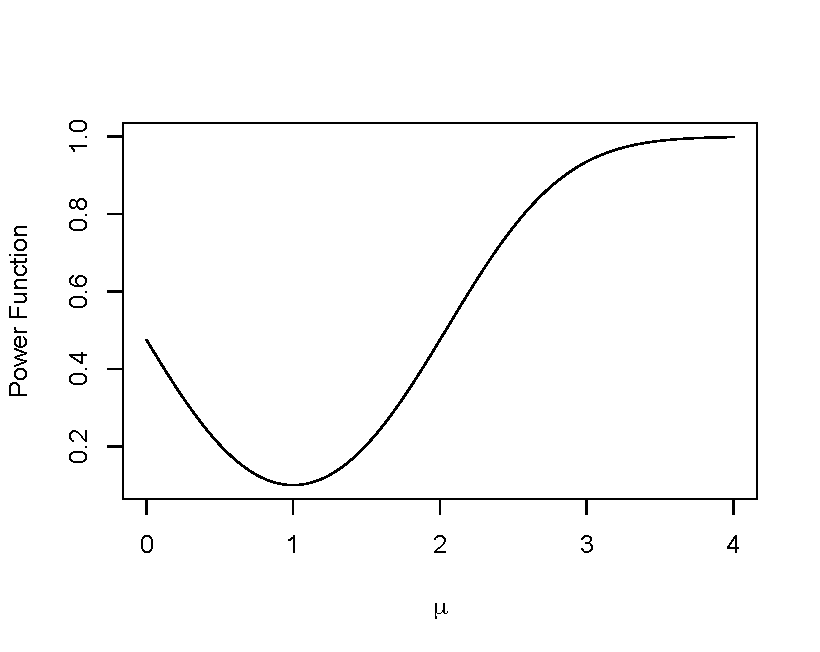
\includegraphics[scale=1]{Powerfun.pdf}
	\newpage
	\item
		To obtain the density of the second order statistic $X_{(2)}$, we use the following identity:
		\[
			f_{X_{(k)}}(x) = k \binom{n}{k}[F(x;\mu)]^{k-1}[1-F(x;\mu)]^{n-k}f(x;\mu)
		\]
	Therefore
		\begin{align*}
			f_{X_{(2)}}(x) &= 2 \binom{10}{2}[F(x;\mu)]^{2-1}[1-F(x;\mu)]^{10-2}f(x;\mu)\\
			&=  2 \frac{10!}{2!8!}[F(x;\mu)][1-F(x;\mu)]^{8}f(x;\mu)\\
			&=\frac{10!}{8!}[F(x;\mu)][1-F(x;\mu)]^{8}f(x;\mu)\\
		\end{align*}
	also it is given that $f(x;\mu) = \frac{1}{2\sqrt{2\pi}}e^{-\frac{(x-\mu)^2}{8}}$, we also know that
		\[
			\frac{X_i-\mu}{2} \sim N(0,1)
		\]
	for all $i = 1,2,...,10$
	\begin{align*}
		F(x;\mu) &= P[X_i<x]\\
		&= P\bigg[\frac{X_i-\mu}{2}<\frac{x_i-\mu}{2}\bigg]\\
		&= \Phi\bigg(\frac{x-\mu}{2}  \bigg)
	\end{align*}
	Therefore, the density of the 2nd order statistic $X_{(2)}$ is
	\begin{align*}
		f_{X_{2}}(x;\mu) = \frac{90}{2\sqrt{2\pi}}e^{-\frac{1}{8}(x-\mu)^2}\bigg[\Phi\bigg( \frac{x-\mu}{2} \bigg)  \bigg]\bigg[1-\Phi\bigg( \frac{x-\mu}{2} \bigg)  \bigg]^8
	\end{align*}
	and under $H_0: \mu =1$
	\[
		f_{X_{2}}(x;1) = \frac{45}{\sqrt{2\pi}}e^{-\frac{1}{8}(x-1)^2}\bigg[\Phi\bigg( \frac{x-1}{2} \bigg)  \bigg]\bigg[1-\Phi\bigg( \frac{x-1}{2} \bigg)  \bigg]^8
	\]
	Then by using the following R command:
	\begin{verbatim} 
  		> fun=function(x){(45/sqrt(2*pi))*exp(-(x-1)^2/8)*pnorm((x-1)/2)*(1-pnorm((x-1)/2))^8}
		> integrate(fun, -Inf, 0)
		0.8635273 with absolute error < 8.3e-09	
	\end{verbatim}
	As a result we found that
		\[
			P(X_2<0)= 0.8635273
		\]
        \end{enumerate}
\newpage
\section*{Question 2}
	\begin{enumerate}[(a)]
	\item 
		Firstly we note that $N_1,...,N_T$ are all $i.i.d$ random variable with common density being $Poisson(\lambda)$ so
			\begin{align*}
				f_{N_i|\Lambda}(n_i|\lambda) = e^{-\lambda} \frac{\lambda^n}{n!} 
			\end{align*}
		The conditional joint density of ${\bold N}$ is
		 \begin{align*}
				f_{N_1,N_2,...,N_n|\Lambda}(n_1, n_2,...,n_n|\lambda) &= \prod^T_{i=1}f_{N_i|\Lambda}(n_i|\lambda) \\
				&=\frac{e^{-\lambda T}\lambda^{\sum^T_{i=1}n_i}}{\prod^T_{i=1}n_i!}
		\end{align*}
		The prior distribution on $\Lambda$ is $Gamma(a,b)$ with known $a>0, b>0$:
			\begin{align*}
				\tau(\lambda) = \frac{\lambda^{a-1}e^{-\lambda/b}}{\Gamma(a)b^a} , \lambda >0
			\end{align*}
		Using both of the given information from above we can deduce that for $N =(N_1,N_2,...,N_n)$ given $\lambda$:
			\begin{align*}
				h(\lambda|N) &\propto f(N|\lambda)\tau(\lambda)\\
				&= \frac{e^{-\lambda T}\lambda^{\sum^T_{i=1}n_i}}{\prod^T_{i=1}(n_i!)}\frac{\lambda^{a-1}e^{-\lambda/b}}{\Gamma(a)b^a} \\
				&= \frac{\lambda^{\sum^T_{i=1}n_i+a-1}e^{-\lambda(T+1/b)}}{\Gamma(a)b^a\prod^T_{i=1}(n_i!)}\\
				h(\lambda|N) &\propto  \lambda^{\sum^T_{i=1}n_i+a-1}e^{-\lambda(T+1/b)} 
			\end{align*}
		which means that $\lambda|N \sim Gamma (\sum^T_{i=1}n_i+a, \frac{1}{T+1/b})$.\\
		Then by applying the Expected value property of the Gamma function, the Bayes estimator of $\lambda$ with respect to quadratic loss is given as follow
			\begin{align*}
			E[\lambda|N] = \frac{\sum^T_{i=1}n_i+a}{T+1/b}\\
			\end{align*}
		\item
			Assume $a=3, b=2$, if the counts within the last sever years were 2, 4, 7,  3, 4, 4, 5, then we also know that $\sum^7_{i=1}n_i =2+4+7+3+4+4+5= 29$\\
			Therefore the estimate of $\lambda$ for this data
			\[
				E[\lambda|N] = \frac{29+3}{7+\frac{1}{2}} = \frac{64}{15} \approx 4.2666667
			\]
		\item
			Assuming $a=3, b=2,T=3$ and using the fact that $\sum^7_{i=1}n_i = 29$, we can found the posterior distribution with respect to $\lambda$ as follow 
			\[
				h(\lambda|N) = \frac{\lambda^{31}e^{-\lambda/7.5}}{\Gamma(32)(1/7.5)^{32}}
			\]
		To test for the statement "the yearly intensity $\lambda$ is less than 4", we can construct a hypothesis test as follow
		\[
		H_0:\lambda <4 \mbox{ vs } H_1: \lambda \ge 4
		\]
		Using the Bayesian testing with a zero-one loss. We then calculate posterior probability given the sample as follow
		\[
		P(\lambda \in \Lambda_0 | N) = \int^4_0 \frac{\lambda^{31}e^{-\lambda/7.5}}{\Gamma(32)(1/7.5)^{32}} d\lambda= 0.0.381357
		\]
		which is calculated using the following R code:
		\begin{verbatim} 
			> pgamma(4,32,15/2)
			[1] 0.381357
		\end{verbatim} 
		As a result we reject $H_0$ since the posterior probability is less than $\frac{1}{2}$. Therefore, we can conclude that the statement claimed by the bank is false. 
	\end{enumerate}
	\newpage
	\section*{Question 3}
	\begin{enumerate}[(a)]
	\item
		\begin{verbatim}
			> #Question 3
> #Part a
> #myskewness
> mkskewness = function(x){
+ 	n= length(x)
+ 	res= x - mean(x)
+ 	numerator = sqrt(n)*sum(res^3)
+ 	denominator = (sum(res^2))^(3/2)
+ 	skew=numerator/denominator
+ 	return(skew)
+ 	}
> #mykurtosis
> mykurtosis = function(x){
+ 	n=length(x)
+ 	res = x-mean(x)
+ 	numerator = n*sum(res^4)
+ 	denominator = (sum(res^2))^2
+ 	kurtosis = numerator/denominator -3
+ 	return(kurtosis)
+ 	}
\end{verbatim}
\item
\begin{verbatim}
> #Part b)
> time = lung[,2]
> myskewness (time)
[1] 1.086788
> skewness(time)
[1] 1.093999
> kurtosis(time)
[1] 0.9401333
> mykurtosis(time)
[1] 0.8934417

\end{verbatim}
By observing the above output, we observe that there is a difference between the output value between "myskewness", "mykurtosis" and "skewness", "kurtosis".\\
Therefore, we obtain a different value for "myskewness()", "mykurtosis()" compare to "skewness()", "mykurtosis()".\\
However, by changing the method argument to "moment", "skewness(,method = "moment")", "mykurtosis(,"moment")" ,we then obtain the same numerical result as "myskewness()", "mykurtosis()".
\begin{verbatim}
> skewness(time, method="moment")
[1] 1.086788
> kurtosis(time, method="moment")
[1] 0.8934417
\end{verbatim} 
An explanation of this can be found from the help of the in-built functions. We notice that there is an optional arguments for "method" which can take in either "fisher" for Fisher's g1(skewness) and g2 (kurtosis) version, and "moment " for the functional forms of the statistic.\\
Since the default option is "fisher", then when we obtain the value using "skewness" and "kurtosis" without specifying the method argument, we are essentially calculating Fisher's g1 and g2 estimates. Therefore, when we specify "moment" in the "method" argument, we will obtain the same value as our own functions.
\item
The code for Bootstrap the $\hat{\gamma}_1$ and $\hat{\gamma}_2$ estimators by using B = 2000 replicates is provided below. Then the output containing the 95\% confidence interval using the BCa method is also shown below:
\begin{verbatim}
> #Part c)
> boot.obj1<-bootstrap(time,myskewness(time),B=2000)
> boot.obj2<-bootstrap(time,mykurtosis(time),B=2000)
> summary(boot.obj1)
Call:
bootstrap(data = time, statistic = myskewness(time), B = 2000)
Number of Replications: 2000
Summary Statistics:
Observed Mean Bias SE 
Param 1.087 1.074 -0.01233 0.1402
Percentiles:
2.5% 5% 95% 97.5% 
Param 0.7974 0.8453 1.312 1.35
BCa Confidence Intervals:
2.5% 5% 95% 97.5% 
Param 0.8319 0.87 1.337 1.387
> summary(boot.obj2)
Call:
bootstrap(data = time, statistic = mykurtosis(time), B = 2000)
Number of Replications: 2000
Summary Statistics:
Observed Mean Bias SE 
Param 0.8934 0.8552 -0.03819 0.4973
Percentiles:
2.5% 5% 95% 97.5% 
Param -0.02609 0.09735 1.715 1.931
BCa Confidence Intervals:
2.5% 5% 95% 97.5% 
Param 0.09131 0.2115 1.923 2.159
\end{verbatim}
According to the output, the 95\% BCa confidence intervals for the skewness is $(0.8319, 1.387)$ and the 95\% BCa confidence intervals for the kurtosis is $(0.09131, 2.159)$.
\newpage
\item
Since both of the confidence interval for skewness and kurtosis exclude 0, we can conclude that the normality of the lung data is in doubt. The normal quantile-quantile plot is not close to a straight line, which confirms the conclusion that was made before that the lung data may not be normally distributed. We can also observe that the data is skewed as the dot does not form a straight line and the kurtosis is clearly not a straight line, therefore, it confirms with the conclusion again.\\
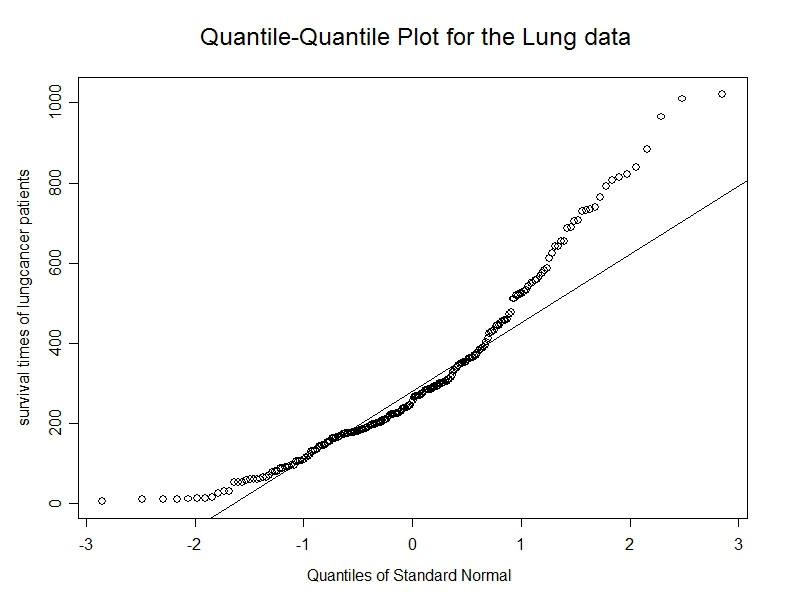
\includegraphics[scale=0.5]{qqplot.jpg}
\begin{verbatim}
> #Part d)
> qqnorm(time, ylab="survival times of lungcancer patients", main="Quantile-Quantile Plot
> for the Lung data")
> qqline(time)
\end{verbatim}
\end{enumerate}
\newpage
\section*{Question 4}
\begin{verbatim}
> set.seed(round(log(3332883)))
> x70 <- runif(70, 0.5, 4)
> e70 <- rnorm(70, mean = 0, sd = 0.2)
> y70 <- 2 + x70 + e70
> x30 <- rnorm(30, mean = 6, sd = 0.5)
> y30 <- rnorm(30, mean = 3, sd = 0.5)
> x <- c(x70, x30)
> y <- c(y70, y30)
> simuldata <- data.frame(x, y)
\end{verbatim}
\begin{enumerate}[i)]
\item {\bf Graph 1:}\\
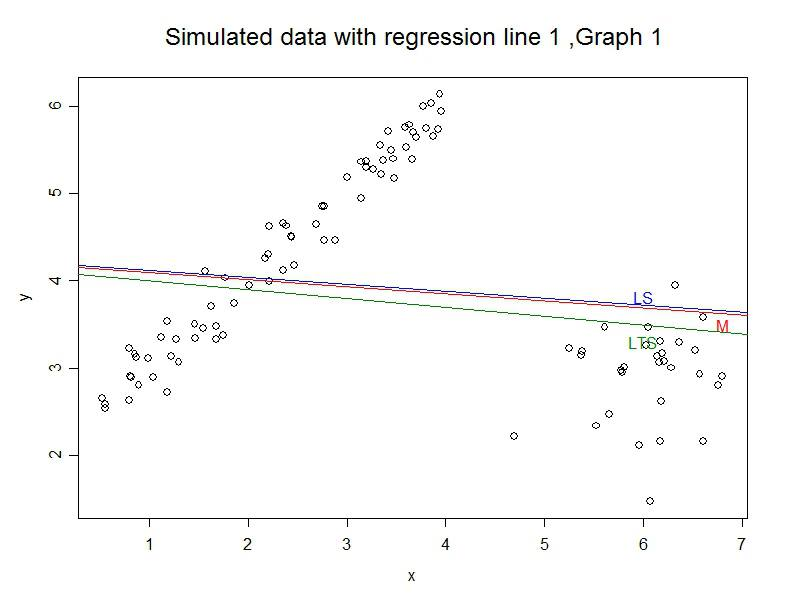
\includegraphics[scale=0.5]{g1.jpg}
\\R code:
\begin{verbatim}
> plot(x, y, main = "Simulated data with regression line 1 ,Graph 1")
> abline(lm(y ~ x, simuldata), col = "blue")
> text(6, 3.82, "LS", col = "blue")
> abline(rreg(x, y), col = "red")
> text(6.8, 3.5, "M", col = "red")
> abline(ltsreg.formula(y ~ x, simuldata), col = "green")
> text(6, 3.3, "LTS", col = "green")
\end{verbatim}
\newpage
\item {\bf Graph 2:}\\
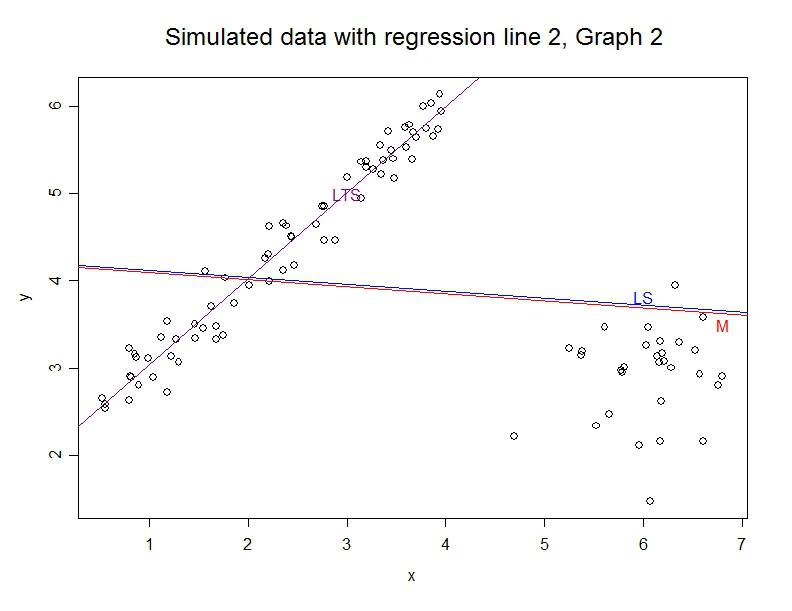
\includegraphics[scale=0.5]{g2.jpg}
\\R code:
\begin{verbatim}
> #line 2
plot(x, y, main = "Simulated data with regression line 2, Graph 2")
> abline(lm(y ~ x, simuldata), col = "blue")
> text(6, 3.82, "LS", col = "blue")
> abline(rreg(x, y), col = "red")
> text(6.8, 3.5, "M", col = "red")
> abline(ltsreg.formula(y ~ x, simuldata, quan = 70), col = "purple")
> text(3, 5, "LTS", col = "purple")
\end{verbatim}
\newpage
\item {\bf Graph 3:}\\
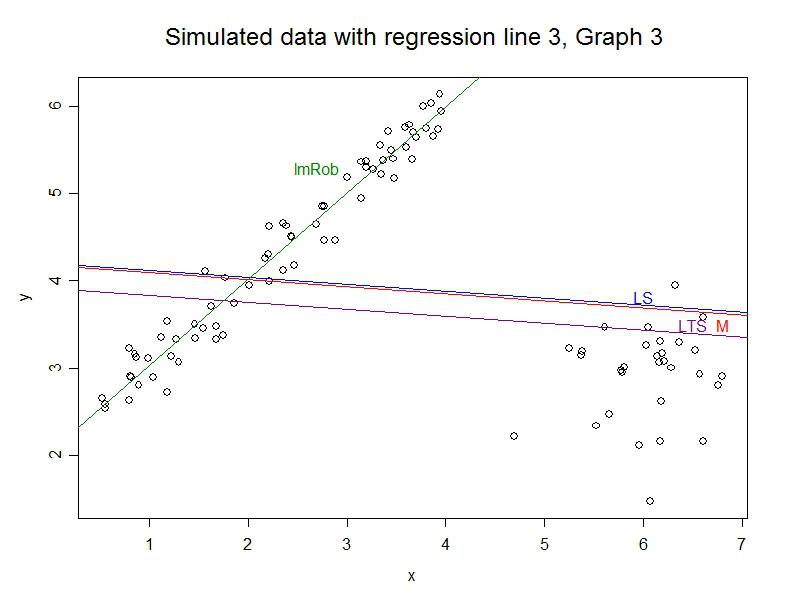
\includegraphics[scale=0.5]{g3.jpg}\\
R code:
\begin{verbatim}
> #lmRob, with residual = 85
plot(x, y, main = "Simulated data with regression line 3, Graph 3")
> abline(lm(y ~ x, simuldata), col = "blue")
> text(6, 3.82, "LS", col = "blue")
> abline(rreg(x, y), col = "red")
> text(6.8, 3.5, "M", col = "red")
> abline(ltsreg.formula(y ~ x, simuldata, quan = 85), col = "purple")
> text(6.5, 3.5, "LTS", col = "purple")
> abline(lmRob(y ~ ., simuldata), col = "green")
> text(2.7, 5.3, "lmRob", col = "green")
\end{verbatim}
Comment: \\
The LTS estimator with 85 residuals consider most of the residuals when plotting the line. In this case, we can observe that , from the graph, using 85 residuals will not  deliver a good fit compare to the previous one which only contains 70 residuals.\\
In LTS, the regression line is fitted by minimising the sum of squares of the m smallest residuals, where m<n. That is, by minimising the objective function
\[
S_{LTS} = \sum^m_{i=1} |e_{(i)}|^2
\]
This method is robust to outliers as the largest n-m outliers do not affect the function $S_{LTS}$.\\
In part i), all three regression lines were highly influenced by outliers. Even LTS was not sufficiently robust as by default, m=90 was chosen, which was too high since 20 clear outliers were included. In part ii), m=70 was chosen, which removed the effect of the 30 clear outliers. This resulted in a more accurate representation of the model. In part iii), m=85 was chosen , which was higher than 70 and lower than 90, as a result it still include 15 clear outliers. Therefore, it produced lines that were highly influenced by outliers.\\
However, the lmRob procedure produced a better fit which is the green line in the above graph. As it is similar to the previous line which used 70 residuals, this suggested that the lmRob does actually adjust "automatically" to the amount of contamination after starting with a high-breakdown point estimator. Therefore, the claim could be believed to be true that lmRob can produce a good fit with its default settings.
\end{enumerate}
\newpage
\section*{Question 5}
\begin{enumerate}[a)]
\item
	\begin{enumerate}[i)]
		\item
			Now consider $X_1,X_2,...,X_n$ are i.i.d. uniform $[0,\theta)$ random variable , with following density function:
			\[
				f(x;\theta) = \left\{ 
				\begin{array}{rcl}
				\frac{1}{\theta} & \mbox{for}
				& 0\le x < \theta \\ 0 & \mbox{for} & \mbox{otherwise} \\
				\end{array}\right.
			\]
			and we can find its cumulative distribution as follow
			\[
				F(x;\theta) = \left\{ 
				\begin{array}{rcl}
				0 & \mbox{for} & x<0 \\
				\frac{x}{\theta} & \mbox{for}
				& 0\le x \le \theta \\ 1 & \mbox{for} & \mbox{otherwise} \\
				\end{array}\right.
			\]
		Consider the estimator $T_n=X_{(n)} = max\{X_1,...,X_n\} $ of $\theta$.
		Using the follow identity,
			\[
				f_{X_{(k)}}(y) = k \binom{n}{k}[F(y;\theta)]^{k-1}[1-F(y;\theta)]^{n-k}f(y;\theta)
			\]
		Since $F(x;\theta)$ is a uniform distribution on $[0,\theta)$, we have
			\begin{align*}
				f_{X_{(k)}}(y) &= k \frac{n!}{k!(n-k)!}\bigg(\frac{y}{\theta}\bigg)^{k-1} \bigg( \frac{y}{\theta} \bigg)^{n-k}\frac{1}{\theta}  & \mbox{ for } y\in[0,\theta) \\
				&=   \frac{n!}{(k-1)!(n-k)!}\bigg(\frac{y}{\theta}\bigg)^{k-1} \bigg( \frac{y}{\theta} \bigg)^{n-k}\frac{1}{\theta} 
			\end{align*}
	Let $y= u\theta$,
	\[
		f_{X_{(k)}}(u\theta) =   \frac{n!}{(k-1)!(n-k)!}u^{k-1}  u^{n-k}
	\]
		Compare to the beta distribution $Z \sim Beta(\alpha,\beta)$
			\[
				f(z) = \frac{(\alpha+\beta-1)!}{(\alpha-1)!(\beta-1)!}z^{\alpha -1} (1-z)^{\beta-1}
			\]
	Therefore
		\[
			\theta f_{X_{(k)}}(u\theta)\sim Beta (\alpha = 1 , \beta = n-k+1)
		\]
	Then denote $B\sim Beta (k,n-k+1)$, we can find 
		\begin{align*}
			E[X_{(k)}] &= \int^\theta_0 y f_{X_{(k)}}(y)  dy\\
			&= \int^1_0 u\theta  f_{X_{(k)}}(u\theta )  \theta du & \mbox{ substitute } y = u \theta \\
			&= \theta \int^1_0 u\bigg(\theta  f_{X_{(k)}}(u\theta )  \bigg) du \\
			&=\theta \int^1_0 u  f_{B}(u) du\\
			&= \theta E[B]\\
			&= \frac{k}{k+n-k+1}\theta\\
			&= \frac{k}{n+1} \theta  
		\end{align*}
	Then we can obtain
		\begin{align*}
			E[X_{(n-1)}] =  \frac{n-1}{n+1} \theta  
		\end{align*}
	Using this fact, we proceed to the next part. First we need to find the $bias(JK(T_n))$. It is known that the jackknife estimator of $\theta$ is 
	\[
		JK(T_n) = nT_n - \frac{n-1}{n}\sum^n_{i=1} T^{(i)}_n
	\]
	where $T^{(i)}_n = max\{ X_1, ... , X_{i-1},X_{i+1}\}$ is the $i^{th}$ jackknife replication of $T_n$.\\
	Then if $X_i \ne X_{(n)}$, the  $i^{th}$ jackknife sample $\{ X_1, ... , X_{i-1},X_{i+1},..., X_n\}$ contains $X_{(n)}$. As $X_{(n)}$ was the largest value in the original sample, it must also be the greatest value in the jackknife sample, so $T^{(i)}_n = X_{(n)}$.\\
	If $X_i = X_{(n)}$, the  $i^{th}$ jackknife sample does not contain $X_n$, so the largest value in the jackknife sample must be the second largest value in the original sample. Hence $T^{(i)}_n = X_{(n-1)}$.\\
	Then applying the above 2 cases,
	\begin{align*}
		JK(T_n) &= nT_n - \frac{n-1}{n} \sum^n_{i=1} T_n^{(i)}\\
		&= nX_{(n)} - \frac{n-1}{n}[(n-1)X_{(n)} + X_{(n-1)} ]\\
		&=X_{(n)}\bigg(n - \frac{(n-1)^2}{n}  \bigg) -\frac{n-1}{n}X_{(n-1)}\\
		&=X_{(n)}\bigg(\frac{n^2-n^2 +2n -1}{n}  \bigg) -\frac{n-1}{n}X_{(n-1)}\\
		&= \frac{2n-1}{n}X_{(n)} - \frac{n-1}{n}X_{(n-1)}
	\end{align*}
	\begin{align*}
		E[JK(T_n)] &= \frac{2n-1}{n}X_{(n)} - \frac{n-1}{n}X_{(n-1)}\\
		&= \frac{2n-1}{n} E[X_{(n)}] - \frac{n-1}{n}E[X_{(n-1)}]\\
	\end{align*}
	applying the result we derived before, we know that
	\[
	E[X_{(n)}] =  \frac{n}{n+1}\theta \mbox{ and } E[X_{(n-1)}] =  \frac{n-1}{n+1}\theta
	\]
	Then we get
	\begin{align*}
		E[JK(T_n)] &= \frac{2n-1}{n} \bigg( \frac{n}{n+1}\bigg) \theta - \frac{n-1}{n}\bigg(\frac{n-1}{n+1}\theta \bigg)\\
		&= \frac{\theta}{n+1} \bigg(2n-1 - \frac{(n-1)^2}{n}\bigg)\\
		&=  \frac{\theta}{n(n+1)} \bigg(2n^2-n - n^2+2n -1\bigg)\\
		&= \frac{\theta}{n(n+1)} \bigg(n^2+n-1\bigg)
	\end{align*}
	Then
	\begin{align*}
		bias(JK(T_n))&=E[JK(T_n)]-\theta \\
		&= \frac{\theta}{n(n+1)} \bigg(n^2+n-1\bigg) - \theta \\
		&=\frac{\theta}{n(n+1)} \bigg(n^2+n-1 - n(n+1)\bigg) \\
		&=\frac{\theta}{n(n+1)} \bigg(n^2+n-1 - n^2-n)\bigg) \\
		&= -\frac{\theta}{n(n+1)}
	\end{align*}
	Since 
	\[
	bias(JK(T_n)) = \bigg|-\frac{\theta}{n(n+1)}\bigg|<\bigg|-\frac{\theta}{(n+1)}\bigg|
	\]
	Therefore, the bias of $JK(T_n))$ is of smaller magnitude in comparison to $-\frac{\theta}{(n+1)}$.
\item
	To find $MSE[T_n]$ and $MSE[JK(T_n)]$. We applied a well known identity
	\[
	MSE[X] = Var[X] +(bias[X])^2
	\]
	Applying this identity, we first decompose $MSE[JK(T_n)]$ as follow
	\begin{align*}
	MSE[JK(T_n)] = Var[JK(T_n)] +(bias[JK(T_n)])^2
	\end{align*}
	When we compute $Var[JK(T_n)] = Var[ \frac{2n-1}{n}X_{(n)} - \frac{n-1}{n}X_{(n-1)}]$, it is necessary for us to first obtain $Var[X_{(n)}] ,Var[X_{(n-1)}]$ and $Cov[X_{(n)},X_{(n-1)}]$.\\
	Then, first obtain the joint density of $X_{(n)}$ and $X_{(n-1)}$ using the follow identity
	\begin{align*}	
	f_{X_{(j)},X_{(k)}}(x,y;\theta) =  \left\{ 
				\begin{array}{rcl}
				\binom{n}{k}\binom{k}{j-1}[F_X(x)]^{j-1}[F_X(y)-F_X(x)]^{k-1-j}[1-F_X(y)]^{n-k}f_X(x)f_X(y)& \mbox{for}
				& x\le y \\ 0 & \mbox{for} & \mbox{otherwise} \\
				\end{array}\right.
	\end{align*}
	Applying the above identity we then have
	\begin{align*}	
	f_{X_{(n-1)},X_{(n)}}(u,v;\theta) &=  \left\{ 
				\begin{array}{rcl}
				\binom{n}{n}\binom{n}{n-2}[F_X(u;\theta)]^{n-2}f_X(u;\theta)f_X(v;\theta)& \mbox{for}
				& u\le v \\ 0 & \mbox{for} & \mbox{otherwise} \\
				\end{array}\right.\\
				&=\left\{ 
				\begin{array}{rcl}
				\frac{n!}{n!(n-n)!}\frac{n!}{(n-2)!(n-n+2)!}[F_X(u;\theta)]^{n-2}f_X(u;\theta)f_X(v;\theta)& \mbox{for}
				& u \le v \\ 0 & \mbox{for} & \mbox{otherwise} \\
				\end{array}\right.\\
				&=\left\{ 
				\begin{array}{rcl}
				\frac{n!}{(n-2)!}[F_X(u;\theta)]^{n-2}f_X(u;\theta)f_X(v;\theta)& \mbox{for}
				& u\le v \\ 0 & \mbox{for} & \mbox{otherwise} \\
				\end{array}\right.\\
				&= \left\{ 
				\begin{array}{rcl}
				n(n-1)(\frac{u}{\theta})^{n-2}\frac{1}{\theta}\frac{1}{\theta}& \mbox{for}
				& u\le v \\ 0 & \mbox{for} & \mbox{otherwise} \\
				\end{array}\right. \\
		f_{X_{(n-1)},X_{(n)}}(u,v;\theta) &= \left\{ 
				\begin{array}{rcl}
				\frac{n(n-1)}{\theta^n}u^{n-2}& \mbox{for}
				& u\le v \\ 0 & \mbox{for} & \mbox{otherwise} \\
				\end{array}\right.
	\end{align*}
	Now we can proceed to evaluate $E[X_{(n-1)},X_{(n)}]$
	\begin{align*}
		E[X_{(n-1)},X_{(n)}]&= \int^\theta_0 \int^v_0 uv f_{X_{(n-1)},X_{(n)}}(u,v;\theta) du dv \\
		&= \frac{n-1}{\theta^n} \int^\theta_0 v \int^v_0 nu^{n-1} du dv\\
		&= \frac{n-1}{\theta^n} \int^\theta_0 v [u^n]^v_0 dv\\
		&= \frac{n-1}{\theta^n} \int^\theta_0 v^{n+1} dv\\
		&= \frac{n-1}{\theta^n} \frac{v^{n+2}}{n+2}\bigg|^\theta_0\\
		&= \frac{(n-1)\theta^{n+2}}{(n+2) \theta^n}  \\
		&= \frac{n-1}{n+2}\theta^{2}
	\end{align*}
	Recall what we derive before $E[X_{(n)}] =  \frac{n}{n+1}\theta \mbox{ and } E[X_{(n-1)}] =  \frac{n-1}{n+1}\theta$ then
	\begin{align*}	
		Cov[X_{(n-1)},X_{(n)}] &= E[X_{(n-1)},X_{(n)}] -E[X_{(n)}]E[X_{(n-1)}]\\
		&=  \frac{n-1}{n+2}\theta^{2} -  \bigg(\frac{n}{n+1}\theta\bigg) \bigg(\frac{n-1}{n+1}\theta \bigg)\\
		&= (n-1)\theta^2 \bigg( \frac{1}{n+2} - \frac{n}{(n+1)^2} \bigg)\\
		&= \frac{(n-1)\theta^2}{(n+1)^2(n+2)}\bigg( (n+1)^2 - n(n+2)\bigg)\\
		&= \frac{(n-1)\theta^2}{(n+1)^2(n+2)}\bigg( n^2 +2n +1 - n^2-2n)\bigg)\\
		&=\frac{(n-1)\theta^2}{(n+1)^2(n+2)}
	\end{align*}
	To evaluate $Var[X_{(n)}] $ we can break it down to
	\begin{align*}
		Var[X_{(n)}] &=E[X_{(n)}^2]-E[X_{(n)}]^2 \\
		&= \int^\theta_0 y^2f_{X_{(n)}}(y)dy - (\theta E[B])^2 & \mbox{using part a i) $E[X_{(n)}] = \theta E[B]$ }\\
		&= \theta^2 \int^1_0 u^2 (\theta f_{X_{(n)}}(u\theta)du - (\theta E[B])^2 & \mbox{substitute $y=u\theta$}\\
		&= \theta^2 \int^1_0 u^2 (\theta f_{B}(u)du - (\theta E[B])^2  & \mbox{where $B\sim Beta (k,n-k+1)$}\\
		&= \theta^2  E[B^2]- (\theta E[B])^2\\
		& = \theta^2 (E[B^2]- E[B]^2)\\
		&= \theta^2 Var(B)\\
		&=\theta^2 \frac{k(n-k+1)}{(n+1)^2(n+2)} & \mbox{ since it's $X_{(n)}$, then $k=n$}\\
		Var[X_{(n)}] &= \frac{n\theta^2 }{(n+1)^2(n+2)}
	\end{align*}
	Similarly we can also get
	\[
	Var[X_{(n-1)}]=  \frac{2(n-1)\theta^2 }{(n+1)^2(n+2)}
	\]
	Finally using all the result we derived above to obtain the $Var[JK(T_n)]$
	\begin{align*}
	Var[JK(T_n)]  &=  Var\bigg[\frac{2n-1}{n}X_{(n)} - \frac{n-1}{n}X_{(n-1)}\bigg]\\
	&= \bigg(\frac{2n-1}{n}  \bigg)^2 Var[X_{(n)}] +\bigg(\frac{n-1}{n}\bigg)^2Var[X_{(n-1)}] -2\bigg(\frac{2n-1}{n}  \bigg)\bigg(\frac{n-1}{n}\bigg) Cov[X_{(n-1)},X_{(n)}]\\
	&= \frac{n(2n-1)^2\theta^2 }{n^2(n+1)^2(n+2)}+\frac{2(n-1)^3\theta^2 }{n^2(n+1)^2(n+2)}-\frac{2(2n-1)(n-1)^2\theta^2}{n^2(n+1)^2(n+2)}\\
	&= \frac{n(2n-1)^2+(n-1)^2[2(n-1) - 2(2n-1)]}{n^2(n+1)^2(n+2)}\theta^2\\
	&=  \frac{n(2n-1)^2+(n-1)^2[2n-2 - 4n+2]}{n^2(n+1)^2(n+2)}\theta^2\\
	&=  \frac{(2n-1)^2+(n-1)^2[ -2]}{n(n+1)^2(n+2)}\theta^2\\
	&= \frac{4n^2 -4n+1-2n^2+4n-2}{n(n+1)^2(n+2)}\theta^2\\
	&= \frac{2n^2 -1}{n(n+1)^2(n+2)}\theta^2
	\end{align*}
	Now we can see that
	\begin{align*}
	MSE[JK(T_n)] &= Var[JK(T_n)] + (bias[JK(T_n)])^2 \\
	&=\frac{2n^2 -1}{n(n+1)^2(n+2)}\theta^2  + \bigg( -\frac{\theta}{n(n+1)} \bigg)^2\\
	&=\frac{2n^2 -1}{n(n+1)^2(n+2)}\theta^2  + \frac{\theta^2}{n^2(n+1)^2}\\
	&=\frac{\theta^2}{n^2(n+1)^2}\bigg(\frac{n(2n^2 -1)}{(n+2)}  + 1\bigg)\\
	&=\frac{\theta^2}{n^2(n+1)^2(n+2)}\bigg(2n^3 -n  + n+2 \bigg)\\
	&=\frac{\theta^22(n^3+1)}{n^2(n+1)^2(n+2)}
	\end{align*}
	Then we can also find $MSE(T_n)$ using the result from above
	\begin{align*}
	MSE[T_n] &= Var[T_n] + (bias[T_n])^2\\
	& =  Var[X_{(n)}] + (bias[X_{(n)}])^2\\
	&=  \frac{n\theta^2 }{(n+1)^2(n+2)} + (E[X_{(n)}]-\theta)^2\\
	&=    \frac{n\theta^2 }{(n+1)^2(n+2)} + \bigg( \frac{n}{n+1}\theta-\theta \bigg)^2\\
	&= \frac{n\theta^2 }{(n+1)^2(n+2)} + \bigg( \frac{n-n-1}{n+1}\bigg)^2\theta^2\\
	&= \frac{n\theta^2 }{(n+1)^2(n+2)} + \frac{1}{(n+1)^2}\theta^2\\
	&= \bigg( n  + n+2\bigg)\frac{\theta^2}{(n+1)^2(n+2)}\\	
	&= \frac{2(n+1)\theta^2}{(n+1)^2(n+2)}\\	
	&= \frac{2(n^3+n^2)\theta^2}{n^2(n+1)^2(n+2)}\\	
	\end{align*}
	Therefore for any $sample\mbox{ } size\mbox{ } n>1$:
	\begin{align*}
		1 &<n^2 \\
		n^3+1 &< n^3 + n^2\\
		2(n^3+1)\theta^2 &<2(n^3 + n^2)\theta^2\\
		\frac{2(n^3+1)\theta^2}{n^2(n+1)^2(n+2)} &<\frac{2(n^3 + n^2)\theta^2}{n^2(n+1)^2(n+2)}\\
		MSE[JK(T_n)] &< MSE[T_n] 
	\end{align*}	
	Hence, jackknifing has also reduced the MSE of the estimator $T_n$.
	\end{enumerate}
\item
It is given that the bootstrap-bias adjustment of $T_n$ happens via $2T_n-E_{\hat{F}}[T^*_n] $ where the expectation is calculated under the empirical distribution.\\
In our case, we have $n=3$, this distribution puts equal weights of 1/3 at $X_{(1)}, X_{(2)}$ and $X_{(3)}$.\\
Hence, to calculate $E_{\hat{F}}[T^*_3] $ we need to consider all the possible outcome of resampling from the original set \{$X_{(1)}, X_{(2)},X_{(3)}$\}:
\begin{align*}
	T^*_3 =\left\{ 
			\begin{array}{rcl}   
				X_{(1)}&= max\{X_{(1)}, X_{(1)},X_{(1)}\}& \mbox{with probability } \bigg(\frac{1}{3}\bigg)^3 \\ 
				X_{(2)}&= \left\{ \begin{array}{rcl}   
							 max\{X_{(1)}, X_{(1)},X_{(2)}\} \\
							max\{X_{(1)}, X_{(2)},X_{(1)}\}\\
							\hdots \hdots  \\
							max\{X_{(2)}, X_{(1)},X_{(2)}\}\\
							max\{X_{(2)}, X_{(2)},X_{(2)}\}\\
						\end{array}\right.
							& \mbox{with probability } \bigg(\frac{1}{3}\bigg)^3 \\
				X_{(3)}&= \left\{ \begin{array}{rcl}   
							 max\{X_{(1)}, X_{(1)},X_{(3)}\} \\
							max\{X_{(1)}, X_{(2)},X_{(3)}\}\\
							\hdots \hdots \\
							max\{X_{(2)}, X_{(2)},X_{(3)}\}\\
							max\{X_{(2)}, X_{(3)},X_{(3)}\}\\
							max\{X_{(3)}, X_{(3)},X_{(3)}\}\\
						\end{array}\right.
							& \mbox{with probability } \bigg(\frac{1}{3}\bigg)^3 \\			
							\end{array}\right.\\
\end{align*}
Therefore, we can split it to 3 cases according to the above distribution\\
Case 1: $X_{(1)}$ \\
Since the only way to obtain $X_{(1)}$ is to have all $X_{(1)}$ in the resampled set. Therefore there's only 1 possible set that will give us $X_{(1)}$.\\
Case 2: $X_{(2)}$ \\
Any resample sets that contains $X_{(1)}$'s and $X_{(2)}$'s but not $X_{(3)}$ will give us $X_{(2)}$. Therefore, there are $2^3$ ways to rearrange $X_{(1)}$ and $X_{(2)}$ in the sets of 3 with replacement. However, we need to exclude the case $\{X_{(1)}, X_{(1)},X_{(1)}\}$ since it will not give us $X_{(2)}$. Hence, there will be in total $(2^3-1)$ possible sets that will give us $X_{(2)}$.\\
Case 3: $X_{(3)}$ \\
Any resample sets that contains $X_{(1)}$'s and $X_{(2)}$'s and $X_{(3)}$ will give us $X_{(3)}$. Therefore, there are $3^3$ ways to rearrange $X_{(1)}$, $X_{(2)}$ and $X_{(3)}$ in the sets of 3 with replacement. However, we need to exclude the cases where $X_{(3)}$ is not included in other words those that will give us  $X_{(2)}$ or $X_{(1)}$ as a result. Hence, there will be in total $(3^3-2^3-1 +1)$ possible sets that will give us $X_{(2)}$.\\
Finally we can compute
\begin{align*}
	E_{\hat{F}}[T^*_3] &=  (1)\bigg(\frac{1}{3}\bigg)^3 X_{(1)}  +  (2^3-1) \bigg(\frac{1}{3}\bigg)^3  X_{(2)} + (3^3-2^3 +1) \bigg(\frac{1}{3}\bigg)^3 X_{(3)}\\
	&= \frac{1}{27} X_{(1)}  +   \frac{7}{27}  X_{(2)} + \frac{19}{27} X_{(3)}\\
\end{align*}
Hence the bootstrap bias-adjusted estimator of $\theta$ is 
\begin{align*}
	2T_3-E_{\hat{F}}[T^*_3] &= 2X_{(3)}-E_{\hat{F}}[T^*_3]  \\
	&= 2X_{(3)}-\bigg( \frac{1}{27} X_{(1)}  +   \frac{7}{27}  X_{(2)} + \frac{19}{27} X_{(3)}\bigg) \\
	&= \bigg(2-\frac{19}{27} \bigg)X_{(3)}-   \frac{7}{27}  X_{(2)}  -  \frac{1}{27} X_{(1)}  \\
	&\approx 1.2963X_{(3)}-   0.25926X_{(2)}  - 0.037 X_{(1)} 
\end{align*}
	Hence we can calculate the bias of the bootstrap bias-adjusted estimator of $\theta$ is then
	\begin{align*}
		bias(\hat{\theta}_{bootstrap\mbox{ }bias-adjusted}) & = E[2T_3-E_{\hat{F}}[T^*_3]] - \theta \\
		&\approx E[1.2963X_{(3)}-   0.25926X_{(2)}  - 0.037 X_{(1)} ] - \theta \\
		&\approx1.2963E[X_{(3)}]-   0.25926E[X_{(2)}]  - 0.037 E[X_{(1)} ] - \theta
	\end{align*}
	From 5 a i), we have derived $E[X_{(k)}] =  \frac{k}{n+1} \theta$ and $n=3$ in our case, therefore we know that 
	\begin{align*}
	E[X_{(1)}] = \frac{1}{4}\theta \mbox{ ,  } E[X_{(2)}] = \frac{2}{4}\theta  \mbox{  , } E[X_{(3)}] = \frac{3}{4}\theta
	\end{align*}
	Then substitute the above expected value to obtain the magnitude of the bias
	\begin{align*}
	|bias(\hat{\theta}_{bootstrap\mbox{ }bias-adjusted})| & \approx \bigg|1.2963 \frac{3}{4} \theta-   0.25926 \frac{1}{2}\theta  - 0.037 \frac{1}{4}\theta - \theta\bigg| \\ 
	& \approx |(-0.166655) \theta| = (0.166655)\theta
	\end{align*}
	Comparing to the magnitude of the bias of the original estimator $T_3$
	\begin{align*}
		|bias(\hat{\theta}_{original})| &= |E(X_{(3)}) - \theta| =\bigg| \theta\bigg[\frac{3}{4}-1\bigg]\bigg|\\
		&= |(-0.25)\theta| = (0.25) \theta\\
		&>(0.166655)\theta = |bias(\hat{\theta}_{bootstrap\mbox{ }bias-adjusted})| 
	\end{align*}
	Hence the bootstrap-based bias adjustment has reduced the magnitude of the bias of the original estimator $T_3$.
\end{enumerate}
\end{document}
